\section{Aufbau und Durchführung \cite{sample}}

\subsection{Dichtebestimmung \label{sec:dichte}}
Zunächst werden die Stäbe gewogen und die Länge $L$ gemessen.
Daraufhin wird beim runden Stab der Radius $r$ und beim eckigen Stab die Seitenlängen $a$, $b$ bestimmt.
Das Volumen $V$ des runden Stabes ist gegeben durch $V=\pi \cdot r^2 \cdot L$,
das des eckigen Stabes hingegen durch $V=a \cdot b \cdot L$.
Die Dichte des jeweiligen Stabes wird dann nach $\rho = \frac{m}{V}$ bestimmt.
\subsection{Einseitige Einspannung \label{sec:einseitig}}
\begin{figure}
  \centering
  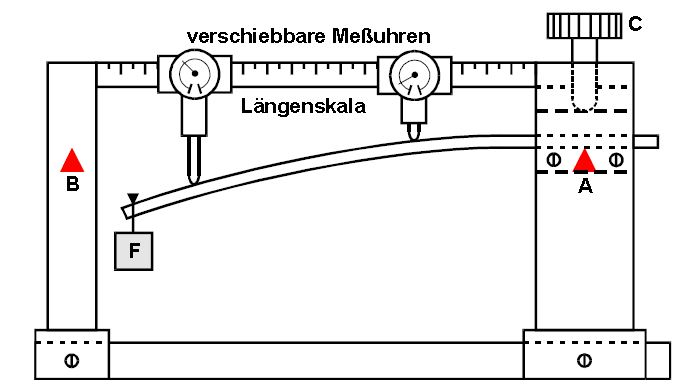
\includegraphics[width=\textwidth]{Text/Aufbau.jpg}
  \caption{Aufbau \cite[2]{sample}}
  \label{fig:Aufbau}
\end{figure}
Einer der beiden Stäbe wird nun enstprechend der Abbildung (\ref{fig:Aufbau}) eingespannt.
Danach wird eine der Messuhren zum Einspannpunkt des Stabes geschoben.
Da nicht davon ausgegangen werden kann, dass der Stab 100\%-ig gerade ist und
sich der Stab schon aufgrund seines Gewichtes biegt, wird zunächst eine Nullmessung durchgeführt.
Dazu wird, bevor ein Gewicht angehängt wird, die Ausdehnung $D(x)$ abgelesen.
Um Fehler zu vermeiden, wird direkt danach ein Gewicht ans Ende des Stabes eingehängt,
die Ausdehnung $D(x)$ erneut abgelesen und die Messuhr auf einen Abstand $x$ verschoben.
Dies wird solange wiederholt, bis das Ende des Stabes erreicht wird.
Der Vorgang wird für den anderen Stab wiederholt.
\subsection{Beiseitige Einspannung}
Der runde Stab wird eingespannt und auf den Punkt B aufgelegt.
Ähnlich wie bei der einseitigen Einspannung(\ref{sec:einseitig}) wird nun die Auslenkung $D(x)$ gemessen.
Es sind jedoch folgene Unterschiede zu beachten:
\begin{itemize}
\item An beide Ende des Stabes wird eine Messuhr geschoben.
\item Beide Messuhren werden nur solange verschoben, bis die Mitte des Stabes erreicht wurde.
\item Das Gewicht wird an die Mitte des Stabes gehängt, nicht an das Ende.
\end{itemize}
